\documentclass[11pt]{article}
\usepackage[T1]{fontenc}
\usepackage{lmodern}
\usepackage[margin=1in]{geometry}
\usepackage{microtype}
\usepackage{amsmath,amssymb,amsthm,mathtools}
\usepackage{enumitem,booktabs,array}
\usepackage{xcolor}
\usepackage{tikz}
\usetikzlibrary{arrows.meta,positioning,calc,fit}
\definecolor{linkblue}{RGB}{22,64,95}
\usepackage[colorlinks=true,linkcolor=linkblue,citecolor=linkblue,urlcolor=linkblue]{hyperref}
\hypersetup{pdftitle={One Sample Suffices for Matroid Prophet Inequalities against an Almighty Adversary},pdfauthor={OpenAI}}
\usepackage[nameinlink,capitalise,noabbrev]{cleveref}
\numberwithin{equation}{section}
\newtheorem{theorem}{Theorem}[section]
\newtheorem{proposition}[theorem]{Proposition}
\newtheorem{lemma}[theorem]{Lemma}
\newtheorem{corollary}[theorem]{Corollary}
\theoremstyle{definition}
\newtheorem{definition}[theorem]{Definition}
\newtheorem{remark}[theorem]{Remark}
\DeclareMathOperator{\cl}{cl}
\DeclareMathOperator{\rk}{r}
\DeclareMathOperator{\OPT}{OPT}
\newcommand{\Ex}{\mathbb E}
\newcommand{\Prob}{\mathbb P}
\newcommand{\ind}[1]{\mathbf 1_{\{#1\}}}
\newcommand{\given}{\,\middle|\,}
\setlist[itemize]{topsep=4pt,itemsep=2pt,parsep=0pt}
\setlist[enumerate]{topsep=4pt,itemsep=3pt,parsep=0pt}
\allowdisplaybreaks[1]
\title{One Sample Suffices for Matroid Prophet Inequalities\\against an Almighty Adversary}
\author{OpenAI}
\date{September 23, 2026}
\begin{document}
\maketitle
\begin{abstract}
We prove that one independent sample per element suffices for a constant-competitive prophet inequality on every finite matroid. The guarantee holds even when the arrival-order adversary observes all samples, all online values, and the algorithm's entire random seed. The rule needs no description of the value distributions and achieves the absolute competitive ratio $2^{-310}$.
\end{abstract}
\section{Introduction}

A prophet inequality compares irrevocable online choices with the best
feasible choice after all values are known. Here feasibility is described
by a known finite labeled matroid $M=(E,\mathcal I)$: its independent sets
$\mathcal I$ are closed under taking subsets and satisfy the augmentation
axiom. For a nonnegative vector $v=(v_e:e\in E)$, write
\[
 \OPT_M(v)=\max_{I\in\mathcal I}\sum_{e\in I}v_e.
\]
An online rule observes labels and their values one at a time, and must
accept or reject each label before the next arrival while keeping its
accepted set independent. The value at each label has an unknown
distribution; before arrivals the rule receives one independent sample
from each of these distributions.

We prove a constant guarantee against an \emph{almighty} ordering
adversary. Besides the samples and the entire online value vector, this
adversary sees the rule's complete random seed before choosing the
permutation. The rule is not told that future order. This exposes both
the statistical information and every random choice that might otherwise
protect the online rule from an unfavorable ordering.

\begin{theorem}\label{thm:main}
There is a measurable online selection rule, independent of the value
distributions, with the following property. Let $M=(E,\mathcal I)$ be any
finite known labeled matroid, and let $(S_e,V_e:e\in E)$ be mutually
independent nonnegative real random variables, with $S_e$ and $V_e$ having
the same arbitrary law $D_e$. Assume
$\Ex[\OPT_M(V)]<\infty$. The rule receives exactly the sample vector $S$
before arrivals and uses a seed $R$ independent of $S,V$.

For every measurable permutation rule $\pi$ depending on $M$, the laws
$(D_e)$, $S$, $V$, and $R$, the rule accepts an independent set $A$,
irrevocably deciding at each arrival using only the available history, and
\begin{equation}\label{eq:main}
 \Ex\left[\sum_{e\in A}V_e\right]
       \ge 2^{-310}\Ex[\OPT_M(V)].
\end{equation}
\end{theorem}

The constant is independent of the matroid, its size and rank, and the
distributions. The rule is a finite measurable construction; no
running-time or polynomial independence-oracle guarantee is claimed.
Section~\ref{sec:accounting} proves the stronger constant $2^{-293}$,
leaving slack in the stated bound. We use no distributional description, extra samples, or
randomness concealed from the adversary.

The proof also gives a secretary consequence. In that model the weights
are fixed before any randomness, and the rule observes and rejects a
random initial segment of a uniformly random permutation. After this
prefix, an adversary that sees all weights, the ordered prefix, and the
complete rule seed may rearrange the remaining labels arbitrarily.
Corollary~\ref{cor:secretary} gives a constant guarantee even with this
suffix order. Both results follow from the same fixed-weight guarantee:
after a random set of weights is revealed and its labels sacrificed, the
expected minimum reward over all orders is a constant fraction of the
fixed optimum.

\paragraph{Historical context.}
In the classical single-choice
problem, independent nonnegative values with known distributions admit
a sharp reward fraction of $1/2$; the original work of Krengel and
Sucheston credits Garling for the factor-two bound~\cite{KS77}.
Kleinberg and Weinberg proved the same $1/2$ guarantee for arbitrary matroid
constraints when the distributions are known~\cite{KW12}. Their arrival
model permits the next label to depend on previously revealed values,
without giving the adversary the unseen values.

For unknown distributions, independent labeled samples provide a natural
alternative source of information. Azar, Kleinberg, and Weinberg developed
this limited-information framework and a reduction from order-oblivious
secretary algorithms to single-sample prophet algorithms~\cite{AKW14}.
In the single-choice setting, Rubinstein, Wang, and Weinberg obtained the
optimal one-sample reward fraction $1/2$~\cite{RWW20}. Caramanis et al.
developed greedy-ordered selection and a pointwise sample-pair framework
for single-sample guarantees under structured feasibility
constraints~\cite{CDF22}. These works illustrate how symmetry between a
sample and a realized value can replace knowledge of a distribution.

This connection also links sample-based selection to the matroid
secretary problem, introduced by Babaioff, Immorlica, and
Kleinberg~\cite{BIK07}. In that problem the weights are fixed and the
arrival order is uniformly random. Lachish~\cite{Lachish14} and Feldman,
Svensson, and Zenklusen~\cite{FSZ15} obtained guarantees with a doubly
logarithmic loss in the rank. The latter gave an order-oblivious rule,
whose guarantee survives adversarial reordering after its observation
prefix, and derived a one-sample prophet inequality with the same
loss~\cite[Theorem 1.1 and Corollary 1.2]{FSZ15}. Thus one sample already
gave guarantees for general matroids; we obtain a constant independent
of rank under full-seed order selection.
Recent work also obtains constant guarantees for ordinary random-order
matroid secretary selection~\cite{Singla26,Huang26}.
Section~\ref{sec:secretary} compares these results, which retain uniformly
random arrivals throughout, with the full-seed adversarial-suffix
consequence proved here.

For every fixed $0<\delta<1/4$, Fu et al. obtained a reward fraction
$1/4-\delta$ for arbitrary matroids on $n$ elements, using
$O_\delta(\log^4(2+n))$ samples per element~\cite{FLTWWZ24}.
Feldman, Svensson, and Zenklusen subsequently improved the sample dependence
on the ground-set size and rank~\cite{FSZ26}. These latter results allow
an almighty adversary, which observes all random realizations before
choosing the order, including the algorithm's randomness.
The full-seed adversary is the almighty adversary of the greedy
online-contention-resolution framework of Feldman, Svensson, and
Zenklusen~\cite[Section 1.1]{FSZ16}. The distinction between one sample
and a sample budget growing with the matroid remains essential even when
the latter gives a much larger numerical constant.

For a different arrival model, Abdi, Banihashem, Hajiaghayi, and Mittal
give a one-sample $1/2$ matroid prophet guarantee using $O(n^2)$
independence queries~\cite[Theorem 1.3]{ABHM26}. Their order is fixed
independently of the samples, online values, and internal random coins.
Theorem~\ref{thm:main} instead permits the order to depend jointly on all
of them. A bound for every fixed order controls the minimum of expected
rewards, whereas this information pattern requires an expected minimum
of rewards. The two guarantees therefore have different adversary
interfaces, as well as different quantitative and computational bounds.

The density decompositions used below have a classical foundation in
Edmonds's matroid partition theorem~\cite{Edmonds65}. Soto used principal
partitions and their uniformly dense minors for secretary selection in
the random-assignment model~\cite{Soto13}; Santiago, Sergeev, and Zenklusen
subsequently developed that approach without advance knowledge of the
matroid~\cite{SSZ25}. Our density optimizer is applied within each sampled
weight group and incorporated into paths expanded by independent guards.
The layer construction also has a predecessor in the alternating
restriction--contraction minors along sampled spans used by Feldman,
Svensson, and Zenklusen~\cite[Section 3]{FSZ15}. Here the sampled
density expansions and guards produce the flats, and the analysis must
control the expected minimum over orders after all seed information is
exposed.

\paragraph{Proof strategy.}
We work first with a fixed hidden vector of weights. Independent masks
reveal some coordinates, which are then sacrificed. The goal in this
formulation is the expectation of the \emph{minimum over all orders},
not a guarantee for an order chosen independently of the masks. A simple
coordinatewise coupling subsequently transfers this guarantee to the
one-sample model (Section~\ref{sec:setup}).

After rounding weights into geometric levels, the main rule constructs
nested paths of flats, that is, subsets closed under matroid span. The
path index is an auxiliary integer, unrelated to arrival time. Process
weight groups from low to high. For each group, enlarge the incoming
flats to capture revealed labels at high density relative to rank. A
separate sparse mask of revealed labels supplies \emph{guards}, which
enlarge a flat one auxiliary step before those labels enter its nominal
path. Differences between alternate flats give two-step layers. Within
each layer the rule greedily selects labels independent over the earlier
endpoint flat. Nesting makes their union feasible for every arrival
order (Section~\ref{sec:algorithm}).

The proof must show that these layers retain enough valuable rank. Three
losses arise, each requiring a different argument.

First, lower-weight arrivals may block a focal weight group. At a
revealed label's nominal entry step, the \emph{safety test} asks whether
it remains outside the density expansion of the earlier flat together
with all possible lower-weight competitors. Expose the guards backwards in
auxiliary time, so that the nominal flats shrink. A
disjoint-certificate bound shows that a label usually leaves at a step
with substantial conditional exit probability. A second transition,
using the independent mask that governs online eligibility, turns this
exit estimate into an expected safe count
(Section~\ref{sec:safety}). All masks are drawn initially; reverse
exposure analyzes their law without concealing any coins from the
adversary.

Second, the safe labels themselves have been sacrificed. In each layer,
choose an independent set spanning the unsacrificed labels over the
earlier flat and lower-weight competitors. The density inequality bounds
the safe count by the density charge times the total size of these sets,
plus the number of labels left outside their span. A large safe count can
therefore fail to yield rank only if this residual is large. The residual
lies entirely in the sacrificed mask. Such a set can depend on that mask,
so a bound for one fixed set does not suffice. We encode residuals by
the marks at which their labels first become spanned in two sequences
with boundedly many inserted generators. A combinatorial bound controls
all such marked-pivot patterns before the focal group's mask is exposed.
Crucially, its bound depends on the number of inserted generators, not
the number of auxiliary times. A union bound then rules
out large residuals with high probability, giving rank on unsacrificed
labels (Section~\ref{sec:transfer}).

Third, passing from a group's nominal path to the final guarded path
enlarges the layer bases, which can reduce that rank. One common set of generators accounts for all such
expansions. A telescoping conditional-rank identity charges its cost only
once across the entire path. After independent eligibility thinning,
the remaining rank lower-bounds cumulative accepted counts
simultaneously for every permutation. Only then do we average and sum
over weight levels (Section~\ref{sec:accounting}). A separate
single-choice branch covers the case in which the heaviest label is a
substantial part of the optimum.

Section~\ref{sec:secretary} realizes the sacrificed mask as a random
observation prefix and proves the secretary consequence.

\section{A fixed-vector formulation}\label{sec:setup}

Throughout, $M=(E,\mathcal I)$ is a finite labeled matroid. For $X\subseteq E$,
its rank $\rk(X)$ is the maximum size of an independent subset of $X$, and
$\cl(X)=\{e\in E:\rk(X\cup\{e\})=\rk(X)\}$ is its closure.
A flat equals its closure; $X$ spans $A$ when $A\subseteq\cl(X)$.
Write $L=\cl(\varnothing)$ for the set of loops, and put
\[
 \rk(A\mid P)=\rk(A\cup P)-\rk(P),\qquad
 \OPT_M(w)=\max_{I\in\mathcal I}\sum_{e\in I}w_e.
\]
Inside a closure, a rank argument, or a map on flats, a sum of sets denotes
their union. A set is independent over $P$ if its conditional rank over $P$
equals its cardinality. We fix a total order on the labels once and for all.

We first consider a deterministic nonnegative weight vector $w$ that is
initially hidden. Before arrivals, a rule draws a mask $B_0\subseteq E$
independently of $w$ and learns $w$ on $B_0$. It must reject every label in
$B_0$. On other labels it learns the weight at arrival. The mask may be a
function of the rule's complete initial random seed $R$. Let
$A(w,R,\pi)$ denote its accepted set under permutation $\pi$.

\begin{proposition}\label{prop:hidden}
There is a measurable rule in the fixed-vector formulation that is feasible for every
realization and every permutation, and for every $w\in[0,\infty)^E$ satisfies
\begin{equation}\label{eq:hidden-guarantee}
 \Ex_R\left[\min_{\pi}\sum_{e\in A(w,R,\pi)}w_e\right]
 \ge 2^{-293}\OPT_M(w).
\end{equation}
Its revealed mask is selected before any weights are seen.
\end{proposition}

The minimum in \eqref{eq:hidden-guarantee} is inside the expectation.
In particular, an adversary may choose a different order for each seed.
All estimates below are for a fixed $M,w$; we suppress these deterministic
objects in conditional expectations.

Using samples on a sacrificed observation set and realized values on its
complement is the simulation underlying the limited-information reduction
of Azar, Kleinberg, and Weinberg~\cite[Section 3]{AKW14}. Related
sample/value symmetries appear in the paired-draw analyses of
Rubinstein, Wang, and Weinberg~\cite[Section 3]{RWW20} and Caramanis
et al.~\cite[Sections 2 and 6]{CDF22}. Here the mask may depend on the
entire seed, and the transfer must preserve the minimum inside the
expectation. We verify these requirements directly.

\begin{lemma}[One-sample simulation]\label{lem:simulation}
A measurable fixed-vector rule satisfying \eqref{eq:hidden-guarantee} yields
a measurable one-sample rule with the same competitive ratio against the
adversary of Theorem~\ref{thm:main}.
\end{lemma}
\begin{proof}
Draw its entire seed independently of the sample and value vectors $S,V$.
For analysis, define
\[
 w_e^{\mathrm{glue}}=
 \begin{cases}S_e,&e\in B_0(R),\\ V_e,&e\notin B_0(R).\end{cases}
\]
Given any seed, the choices of which copies to use are fixed. The mutual
independence and matching laws of $S_e,V_e$ imply
\[
 \mathcal L(w^{\mathrm{glue}}\mid R)
       =\bigotimes_{e\in E}D_e.
\]
Thus $w^{\mathrm{glue}}$ is independent of the complete seed and has the
law of $V$. Implement the fixed-vector rule using $S_e$ only on its revealed
mask and $V_e$ elsewhere when a label arrives. Ignore unused samples and
reject revealed labels without using their online values. For every fixed
$S,V,R$ and every permutation, induction on arrivals shows that this
execution has exactly the accepted set $A(w^{\mathrm{glue}},R,\pi)$;
each accepted weight is its actual online value.

Consequently, for any adversarial choice of $\pi$, including one depending
on all the unused samples and values, its reward is at least
$\min_{\pi'}\sum_{e\in A(w^{\mathrm{glue}},R,\pi')}w_e^{\mathrm{glue}}$.
Integrate \eqref{eq:hidden-guarantee} using independence of the glued vector
and seed. This gives the desired inequality. Nonnegative integration is
valid without further moment assumptions, and feasibility bounds the
reward by $\OPT_M(V)$, whose expectation is finite.
\end{proof}

\subsection{Elementary matroid facts}

The independent sets contain $\varnothing$, are closed under subsets, and
satisfy augmentation: for $I,J\in\mathcal I$ with $|I|<|J|$, some
$e\in J\setminus I$ has $I\cup\{e\}\in\mathcal I$.
A basis of a set $X$ is a maximal independent subset of $X$.
We use only rank and closure, so the argument applies to nonrepresentable
matroids as well. The augmentation axiom implies that all maximal
independent subsets of a given set have the same size, and that independent
sets extend to bases of larger sets. Rank is submodular:
\begin{equation}\label{eq:rank-submodular}
 \rk(A)+\rk(B)\ge\rk(A\cup B)+\rk(A\cap B).
\end{equation}
Indeed, extend a basis of $A\cap B$ to one of $A$, then to one of $A\cup B$
using elements of $B\setminus A$. The initial intersection basis together
with these last elements is independent in $B$, which proves the inequality.
It follows that $\rk(Z\mid P)$ decreases when $P$ grows. Closure is increasing
and idempotent, and adjoining spanned elements changes neither rank nor
closure. In particular, scanning a set and greedily accepting elements that
increase rank over a fixed base $P$ selects an independent set over $P$
of size $\rk(Z\mid P)$ and spans all of $Z$ over $P$.

\section{Constructing the fixed-vector rule}\label{sec:algorithm}

We construct the rule of Proposition~\ref{prop:hidden} for a fixed hidden
weight vector. It uses geometric rounding and chooses with equal
probability between a single-choice maximum branch and a main branch.
The maximum branch handles weight concentrated on one label. The main
branch filters arriving labels against revealed weights and assigns
eligible arrivals to layers of nested flats constructed from those
revealed weights. Greedy independent sets from different layers can
then be combined feasibly.

\subsection{Rounding and a maximum branch}

Fix the constants
\begin{equation}\label{eq:constants}
 B=2^{32},\qquad \kappa=2^{100},\qquad t=2^{-140},\qquad
 \eta=2^{-12},\qquad \gamma=\eta/16=2^{-16}.
\end{equation}
Here $B$ separates weight levels, $\kappa$ is the rank charge in the
density expansions, and $t$ is the common sparsity of the guard and
eligibility masks. The exit-probability cutoff $\eta$ gives the
sample-to-rank coefficient $\gamma$. The choices leave room for the
losses combined in Section~\ref{sec:accounting}.
For $w_e>0$, round down to $u_e=B^{\lfloor\log_B w_e\rfloor}$, and put
$u_e=0$ when $w_e=0$. Define $u(Z)=\sum_{e\in Z}u_e$ and
$W=\OPT_M(u)$. The rule rounds each coordinate when its weight is
revealed or arrives; the full vector $u$ is used only for analysis. Then
\begin{equation}\label{eq:rounding}
 \OPT_M(w)/B\le W\le\OPT_M(w).
\end{equation}
Larger rounded weights have higher priority, with ties resolved by the fixed
label order. Priority greedy on all positive labels produces an independent
set $I^*$ of weight $W$: its intersection with every initial segment of
weight levels has full rank there, so summing the differences of successive
levels proves optimality.

Let $m_*$ be the largest rounded weight of a positive nonloop, or zero if
there is none. A \emph{maximum rule} reveals a fair independent mask and
accepts the first unmasked positive nonloop of higher priority than every
revealed positive nonloop, then accepts nothing further. If there are at
least two positive nonloops, with probability $1/4$ the highest-priority
one is unmasked and the second is masked. On this event only the highest
can exceed the threshold, so it is accepted in every order. With one
positive nonloop, success has probability $1/2$. Thus in all cases
\begin{equation}\label{eq:maximum}
 \Ex\big[\min_\pi u(A_{\mathrm{max}}(R,\pi))\big]\ge m_*/4.
\end{equation}
The final fixed-vector rule uses this rule or the main rule constructed
next, with equal probability. The maximum branch gives the guarantee when
the largest rounded weight is large enough relative to the rounded optimum;
the main branch handles the complementary case. Draw all coins, including unused branch
coins, initially and independently of the weights.

\subsection{Candidates and weight groups}

For the main rule draw mutually independent masks $H,D,C,T$, independently
across labels, with respective membership probabilities $1/2,1/4,t,t$.
Their roles are summarized below.
\begin{center}
\begin{tabular}{@{}ccl@{}}
\toprule
Mask & Probability & Role \\
\midrule
$H$ & $1/2$ & Filters candidates by higher-priority span \\
$D$ & $1/4$ & Lists weight groups and supplies density data \\
$C$ & $t$ & Supplies guards for the flat paths \\
$T$ & $t$ & Thins online eligibility independently of the paths \\
\bottomrule
\end{tabular}
\end{center}
Reveal the fixed-vector weights on $H\cup D\cup C$
and sacrifice these labels. Under Lemma~\ref{lem:simulation}, these revealed
weights are the corresponding sample coordinates.
Membership in $T$ alone reveals no weight and forces no rejection.
For each label $e$, let $H_{>e}$ be the labels in $H$ with higher priority
than $e$. Define the candidate set and a comparison independent set by
\begin{equation}\label{eq:candidates}
 U=\{e\notin H:u_e>0,\ e\notin\cl(H_{>e})\},
 \qquad Y=I^*\setminus H.
\end{equation}
The full set $U$ is used for analysis; the candidate test itself is
computable as soon as the weight of $e$ is known.

\begin{lemma}[Candidate mass]\label{lem:filter}
The set $Y$ is independent, $Y\subseteq U$, and
\begin{equation}\label{eq:candidate-mass}
 \Ex_H u(Y)=W/2,\qquad \Ex_H u(U)\le W.
\end{equation}
\end{lemma}
\begin{proof}
For $e\in I^*$, no higher-priority labels span $e$, so neither do the
higher-priority labels of $H$. This proves $Y\subseteq U$; its expectation
follows from the fair mask. Conditional on all higher-priority memberships
in $H$, the event $e\notin\cl(H_{>e})$ is fixed. Its contribution to $u(U)$
has the same expected weight as the event that $e$ belongs to $H$ and is
selected by priority greedy on $H$. Sum over the positive labels.
The resulting expected greedy weight on $H$ is at most $W$.
\end{proof}

Conditional on $H$, the \emph{true weight groups}
\[
 U_i=\{e\in U:u_e=B^i\},\qquad n_i=|U_i|,\qquad Y_i=Y\cap U_i
 \quad(i\in\mathbb Z)
\]
are fixed. Empty groups may be omitted. A group is \emph{listed} when
$D\cap U_i\ne\varnothing$. Enumerate the listed groups as $G_1,\ldots,G_m$
from lower to higher weight, and write $D_h=D\cap G_h$, $C_h=C\cap G_h$,
and $T_h=T\cap G_h$. The complete $D_h,C_h$ are known before arrivals:
every label of $D\cup C$ is revealed, and its candidate test uses only $H$
and its own weight. The algorithm needs neither the complete $G_h$ nor
the true group sizes $n_i$. All candidates are nonloops.

\subsection{Density expansions}

For a listed group $h$ and a flat $P$, let $Q_h(P)$ be the largest flat
maximizing
\begin{equation}\label{eq:density-objective}
 f_h(Z)=|D_h\cap Z|-\kappa\rk(Z)
 \qquad\text{over flats }Z\supseteq P.
\end{equation}
For a nonflat argument, take its closure first. The objective rewards the
number of $D_h$ labels spanned and charges $\kappa$ per unit of rank.
Comparison with a further extension bounds its additional sample count
by $\kappa$ times its additional rank. A separate telescoping argument in
Lemma~\ref{lem:generators} bounds the generators used over the entire path.

This is a contracted, sample-restricted form of the cardinality-minus-rank
maximization associated with principal partitions; see Santiago, Sergeev,
and Zenklusen~\cite[Section 3.1, Equation (1)]{SSZ25}. We prove the needed
monotonicity and residual-rank bounds directly.

\begin{lemma}[Density expansion]\label{lem:density}
The largest maximizer in \eqref{eq:density-objective} exists, the map $Q_h$
is increasing, and $P\subseteq Q_h(P)$. If $Q=Q_h(P)$, then for every set $Z$,
\begin{equation}\label{eq:density-residual}
 |D_h\cap(\cl(Q+Z)\setminus Q)|\le\kappa\rk(Z\mid Q).
\end{equation}
\end{lemma}
\begin{proof}
The function $f_h$ is supermodular on the lattice of flats: the counting
term is supermodular under intersection and closed union, and the negative
rank term is supermodular by \eqref{eq:rank-submodular}. There are finitely
many flats. The closed union of any two maximizers containing $P$ is again
a maximizer, so there is a largest one.

For $P\subseteq P'$, put $Q=Q_h(P)$ and $Q'=Q_h(P')$. The flat
$Q\cap Q'$ is feasible at $P$ and $\cl(Q\cup Q')$ is feasible at $P'$.
Optimality gives one inequality and supermodularity the reverse:
\[
 f_h(Q\cap Q')+f_h(\cl(Q\cup Q'))
       \le f_h(Q)+f_h(Q')
       \le f_h(Q\cap Q')+f_h(\cl(Q\cup Q')).
\]
Equality in the two optimality comparisons shows that $\cl(Q\cup Q')$
is also a maximizer at $P'$. Its largest maximizer contains $Q$, as claimed.
Finally compare $Q$ with the feasible flat $\cl(Q+Z)$ in
\eqref{eq:density-objective}. The difference of their ranks is
$\rk(Z\mid Q)$, giving \eqref{eq:density-residual}.
\end{proof}

\subsection{Nominal paths and guards}

Integer $k$ denotes an \emph{auxiliary time}, unrelated to arrival time.
Set $F_0(k)=L$ for $k<0$ and $F_0(k)=E$ for $k\ge0$. For each listed group,
put $a_h=-3h$ and define an enabled expansion
\[
 Q_{h,k}(P)=
 \begin{cases}Q_h(P),&k\ge a_h,\\ P,&k<a_h,\end{cases}
 \qquad(P\text{ a flat}).
\]
In increasing group order, form its \emph{nominal} and \emph{guarded} paths
\begin{equation}\label{eq:paths}
 X_h(k)=Q_{h,k}(F_{h-1}(k)),\qquad
 F_h(k)=\cl\bigl(X_h(k)+(C_h\cap X_h(k+1))\bigr).
\end{equation}
Thus a guard uses a label one auxiliary step before it enters the nominal
path. Each density map uses only $D_h$ and the known matroid, and each
guard set uses the revealed labels $C_h$. Consequently these flats can
be computed as subsets of $E$ before arrivals, even though the weights
of some labels they contain remain unknown.

\begin{lemma}[Path properties]\label{lem:paths}
The paths increase with $k$ and satisfy
\begin{equation}\label{eq:path-inclusions}
 F_{h-1}(k)\subseteq X_h(k)\subseteq F_h(k)\subseteq X_h(k+1).
\end{equation}
They equal $E$ for $k\ge0$. Moreover $X_h(k)=L$ for $k<a_h$ and
$F_h(k)=L$ for $k<a_h-1$. If $e$ is a nonloop, its nominal birth
\[
 b_h(e)=\min\{k:e\in X_h(k)\}
\]
is either $a_h$, with $e\in Q_h(L)$, or belongs to $[a_h+2,0]$.
\end{lemma}
\begin{proof}
Induct on $h$. The map $Q_{h,k}$ is increasing both in its argument and
in $k$, since enabling it replaces the identity by an extensive increasing
map. Thus $X_h$ and then $F_h$ are increasing. The first two inclusions
in \eqref{eq:path-inclusions} are extensiveness; the last follows because
both sets adjoined in the definition of $F_h(k)$ lie in the flat $X_h(k+1)$.
The same recursion gives $E$ at times at least zero.

For $h>1$, $a_{h-1}=a_h+3$ and the inductive lower bound makes
$F_{h-1}(k)=L$ for $k<a_h+2$; this also holds for $h=1$ directly from
$F_0$. Before $a_h$ the new map is the identity, proving the asserted
lower bounds for $X_h$ and $F_h$. At $a_h$ and $a_h+1$, the nominal flat
is the same flat $Q_h(L)$, so no nonloop is born at $a_h+1$.
\end{proof}

\subsection{The online decisions}

Choose an independent fair parity $\varepsilon\in\{0,1\}$ and put
$\widehat F(k)=F_m(k)$. When $m=0$, use $\widehat F=F_0$ and reject all
arrivals. In general the layer endpoints are the integers
$b\equiv\varepsilon\pmod2$, with layer $(b-2,b]$ having base
$\widehat F(b-2)$.
The rule maintains a set $A_b\subseteq\widehat F(b)$ in each layer,
independent over its base $\widehat F(b-2)$.
Since successive layers share an endpoint, all labels selected in an
earlier layer lie in the base of every later layer. Greedy selection in
alternating restriction--contraction minors also appears in
Feldman, Svensson, and Zenklusen~\cite[Section 3]{FSZ15}; here the nested
flats come from the guarded density paths.

At arrival of a label $e$, perform the following operations.
\begin{enumerate}
 \item Reject if $e\in H\cup D\cup C$, if its candidate test fails,
 or if its rounded weight is not listed.
 \item For its listed group $h$, compute $b=b_h(e)$. Reject unless
 \begin{equation}\label{eq:eligibility}
 e\in T,\qquad b\ge a_h+2,\qquad b\equiv\varepsilon\pmod2,
 \qquad e\notin\widehat F(b-2).
 \end{equation}
 \item Let $A_b$ be the previously accepted labels assigned to this
 layer. Accept $e$ exactly when
 $\rk(\{e\}\mid\widehat F(b-2)+A_b)=1$, and then add it to $A_b$.
\end{enumerate}
These operations use the revealed data, the arriving label and weight,
the seed, and the previous decisions. In particular, no full true weight
group or future arrival is needed.
By Lemma~\ref{lem:paths}, the three-step activation schedule leaves no
birth at $a_h+1$. Excluding the baseline birth $a_h$ therefore leaves exactly
the births for which $b-2\ge a_h$: the density map is already enabled
at the preceding layer endpoint. Figure~\ref{fig:paths} shows both the
guard step and the nesting that makes layerwise decisions feasible.

\begin{figure}[htbp]
\centering
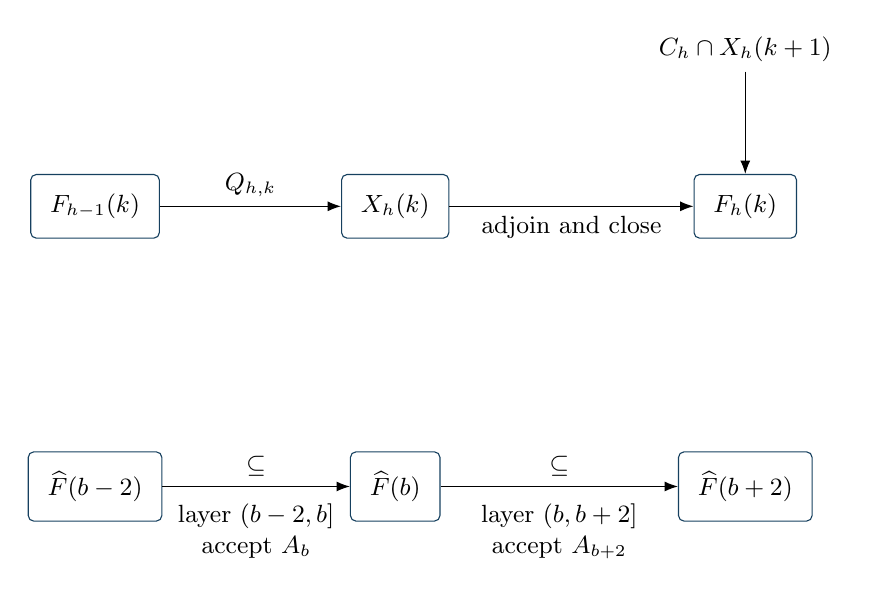
\begin{tikzpicture}[>=Latex, every node/.style={font=\small},
 flat/.style={draw=linkblue,rounded corners=2pt,inner sep=7pt}]
 \node[flat] (prior) {$F_{h-1}(k)$};
 \node[flat,right=23mm of prior] (nominal) {$X_h(k)$};
 \node[flat,right=31mm of nominal] (guarded) {$F_h(k)$};
 \node[above=13mm of guarded] (guard) {$C_h\cap X_h(k+1)$};
 \draw[->] (prior) -- node[above] {$Q_{h,k}$} (nominal);
 \draw[->] (nominal) -- node[below] {adjoin and close} (guarded);
 \draw[->] (guard) -- (guarded);
 \node[flat,below=27mm of prior] (leftbase) {$\widehat F(b-2)$};
 \node[flat,below=27mm of nominal] (middlebase) {$\widehat F(b)$};
 \node[flat,below=27mm of guarded] (rightbase) {$\widehat F(b+2)$};
 \draw[->] (leftbase) -- node[above] {$\subseteq$}
     node[below=1mm,align=center] {layer $(b-2,b]$\\accept $A_b$} (middlebase);
 \draw[->] (middlebase) -- node[above] {$\subseteq$}
     node[below=1mm,align=center] {layer $(b,b+2]$\\accept $A_{b+2}$} (rightbase);
\end{tikzpicture}
\caption{Above: a density expansion followed by guards from the next
nominal time gives $F_h(k)\subseteq X_h(k+1)$. Below: two consecutive
layers of the chosen parity on the final path. The set $A_b$ is
independent over $\widehat F(b-2)$ and lies in $\widehat F(b)$;
$A_{b+2}$ is independent over this latter base. In the lower panel,
the horizontal order is auxiliary time, regardless of the actual
arrival order.}
\label{fig:paths}
\end{figure}

\begin{lemma}[Feasibility and measurability]\label{lem:feasibility}
The main rule maintains an independent accepted set at every arrival
prefix, for every permutation. It is a measurable rule based only on the
allowed information.
\end{lemma}
\begin{proof}
Every eligible label at endpoint $b$ lies in
$X_h(b)\subseteq\widehat F(b)$. The accepted set of its layer is
independent over $\widehat F(b-2)$. In increasing auxiliary endpoint order,
all earlier accepted layers lie in that base flat, so extending by the
current layer preserves independence. This proves independence of the
union for any interleaving of arrivals, and of every prefix.

All masks are drawn initially and the matroid is known. Each density
maximization is over finitely many flats. By Lemma~\ref{lem:paths}, it is
enough to compute a finite interval of integer times for the at most
$|E|$ listed groups. Positive rounding has countably many measurable
level sets; each realized vector has finitely many occupied levels.
All remaining operations are finite rank tests, comparisons, and set
operations with fixed tie rules. They therefore define measurable
decisions. Zeros are never passed to a logarithm, and loops fail the
candidate test.
\end{proof}

\subsection{A generator budget for the entire path}

The rule is now fully specified. To analyze it, we need a bound on how
much each density expansion can change the path. Bounding the rank
increase separately at each time would charge the same sample labels
repeatedly. The next lemma instead chooses one set of generators for all
times. It also bounds the independent sampled mass excluded by the
baseline-birth condition.

\begin{lemma}[A generator budget for the entire path]\label{lem:generators}
For each listed group $h$ there is a set $J_h\subseteq D_h$ and increasing
subsets $J_h(k)\subseteq J_h$ such that
\begin{equation}\label{eq:generator-budget}
 X_h(k)=\cl(F_{h-1}(k)+J_h(k)),\qquad
 |J_h|\le |D_h|/\kappa.
\end{equation}
In particular $\rk(Q_h(L))\le |D_h|/\kappa$.
\end{lemma}
\begin{proof}
Before $a_h$ no generators are needed. Process the enabled times
$k=a_h,a_h+1,\ldots,0$ in order. Given the preceding generators, set
\[
 P_k=\cl(F_{h-1}(k)+X_h(k-1)).
\]
By monotonicity, $P_k\subseteq X_h(k)$. It is feasible in the maximization
defining $X_h(k)$, whence
\begin{align*}
 \kappa\bigl(\rk(X_h(k))-\rk(P_k)\bigr)
 &\le |D_h\cap X_h(k)|-|D_h\cap P_k|\\
 &\le |D_h\cap X_h(k)|-|D_h\cap X_h(k-1)|.
\end{align*}
The flat $R_k=\cl(F_{h-1}(k)+(D_h\cap X_h(k)))$ is contained in
$X_h(k)$ and has exactly the same $D_h$ count. If this inclusion were
proper, $R_k$ would have smaller rank, since a proper subflat has
smaller rank. It would then improve the objective, contradicting
optimality. Thus $R_k=X_h(k)$, and the extension over $P_k$ has a
basis chosen from $D_h\cap X_h(k)$.

Adjoin such a basis to the generators, choosing by the fixed label order.
Since $F_{h-1}$ increases, the preceding generators together with
$F_{h-1}(k)$ already generate $P_k$. This proves the first identity
inductively. The new generators are distinct, and their counts satisfy
the displayed inequality. Summing it telescopes the $D_h$ counts and
gives $|J_h|\le |D_h|/\kappa$. Extend the generator sets constantly
for $k>0$. At $k=a_h$, the lower-group flat is $L$, yielding the last
assertion.
\end{proof}

For the analysis, we first work on a group's own nominal path. The next
section shows that earlier groups' guards protect a constant fraction of
its independent sampled mass against lower-weight competition. We then
transfer this sampled count to unsacrificed rank. Later groups' path
expansions will be paid for by a single rank budget in
Section~\ref{sec:accounting}.

\section{Reverse exposure and safe samples}\label{sec:safety}

The guards from lower-weight groups serve two purposes. They determine
the paths, and they protect a sampled label against lower-weight
competition in its layer. We relate these purposes by exposing the guard
mask backwards in auxiliary time. A label leaves its nominal flat at a
step having a reasonably large conditional exit probability with constant
probability. A comparison using the test mask then turns the square of
that exit probability into a safety guarantee.

Fix $H,D$ and a listed group $h$ throughout this section. Thus the groups,
their indices, the density maps, and $Y$ are fixed. As elsewhere, the
deterministic $M,w$ are suppressed from conditioning. Define
\begin{equation}\label{eq:competition-set}
 K_{h,b}=\bigcup_{j<h}
       \bigl(T_j\cap(X_j(b)\setminus X_j(b-1))\bigr).
\end{equation}
This set contains all possible eligible lower-weight competitors at
endpoint $b$, and is contained in $F_{h-1}(b)$. It includes test-mask
memberships on sacrificed labels; this only enlarges the comparison set.
Let $\sigma_h$ count the labels $d\in D_h\cap Y$ whose birth $b$ on $X_h$
satisfies
\begin{equation}\label{eq:safe-definition}
 a_h+2\le b\le0,\qquad b\equiv\varepsilon\pmod2,\qquad
 d\notin Q_h\bigl(F_{h-1}(b-2)+K_{h,b}\bigr).
\end{equation}
These are analysis quantities; the online rule does not compute them.
Our objective is Lemma~\ref{lem:safe}: a constant fraction of
$D_h\cap Y$ contributes to $\sigma_h$ in expectation, apart from the
loss $|D_h|/\kappa$. We first expose the guards backwards so that each
step queries only previously untouched bits. A bound on disjoint
positive certificates then locates an exit of substantial conditional
probability. Comparing two transitions at that exit will establish the
exclusion in \eqref{eq:safe-definition}.

\subsection{The reverse computation and its filtration}

The guard mask was drawn as part of the initial seed and may be fully known
to the adversary. Reverse exposure analyzes that mask's product law; it
introduces no new online randomness and does not restrict the adversary's
information.

For $k<0$, a later state $S=(S_j:j\le h)$ and a guard-bit vector $c$,
define a one-step map $\mathcal G_k(c,S)$ as follows:
\begin{equation}\label{eq:reverse-map}
 \begin{aligned}
 A_0&=F_0(k),\qquad N_j=Q_{j,k}(A_{j-1}),\\
 A_j&=\cl\bigl(N_j+\{e\in G_j\cap S_j:c_e=1\}\bigr)
       \quad(1\le j\le h).
 \end{aligned}
\end{equation}
Its output is $(N_j:j\le h)$. The map is increasing in $k$, in each
coordinate of $S$, and in the bits $c$, by monotonicity and extensivity of
the density maps. We may view $c$ as a bit vector on the fixed union of
the groups, even though only its restrictions to $G_j\cap S_j$ are used.

Starting with $X_j(0)=E$, compute $X(k)$ at
$k=-1,-2,\ldots,a_h-1$ using
\[
 X(k)=\mathcal G_k(C,X(k+1)).
\]
This is exactly the defining path recursion. For an actual later state
$S=X(k+1)$, the new $N_j$ is contained in $S_j$ for every choice of $c$.
Indeed, inductively $A_{j-1}\subseteq S_{j-1}\subseteq F_{j-1}(k+1)$,
so $N_j\subseteq Q_{j,k+1}(F_{j-1}(k+1))=S_j$; all the guard additions
forming $A_j$ also belong to $S_j$. For $j=1$, use
$F_0(k)\subseteq F_0(k+1)$ to begin the induction.

After computing $N_j$, inspect only the bits on
\begin{equation}\label{eq:departing-query}
 G_j\cap(S_j\setminus N_j).
\end{equation}
The omitted additions inside $N_j$ do not change its closure. Fix a label
order within each such batch. Its domain is determined before its first
query: $N_j$ uses only previous groups' bits. The groups are disjoint and
their domains shrink at each reverse step, so no coordinate is ever
queried twice.

Let $\mathcal H_b$ be the sigma-field generated by the complete transcript
just before the step from $X(b)$ to $X(b-1)$, including the queried labels,
their answers, and the states obtained from them. Thus
$\mathcal H_b\subseteq\mathcal H_{b-1}$ as reverse time advances.
Conditional on $\mathcal H_b$, the unqueried bits on
\[
 V_b=\bigcup_{j\le h}(G_j\cap X_j(b))
\]
are jointly independent Bernoulli bits of rate $t$. Indeed, the
unqueried coordinates are exactly these domains, and each preceding
query was chosen from its prior transcript. In particular, the
conditional transition law is \eqref{eq:reverse-map} with fresh product
bits. The transcript reveals no test bits, parity, or flat at a smaller
time that has not yet been computed.

For a fixed nonloop $d$, on $\{d\in X_h(b)\}$ define the predictable exit
probability
\begin{equation}\label{eq:exit-probability}
 p_{b-1}=\Prob\bigl(d\notin X_h(b-1)\mid\mathcal H_b\bigr).
\end{equation}
Set $p_{b-1}=0$ when $d\notin X_h(b)$. Before exit, these probabilities
are nondecreasing in the order of the reverse computation. To see this,
evaluate each conditional transition probability with an independent
product mask $\xi$ on the whole union of the groups. Smaller time and
smaller input state give a smaller output under this same $\xi$.
Taking probabilities proves the assertion even though the domains of
the unqueried bits change.

\subsection{Certificates and exit mass}

To control exits at steps with $p_{b-1}<\eta$, we consider bands of
comparable exit probabilities. We will show that each survival within a
band certifies one fixed increasing event using only that step's newly
queried positive bits. The next lemma bounds how many such disjoint
certificates can occur.

An increasing Boolean event is a family $\mathcal A\subseteq2^V$ closed
under taking supersets. A positive certificate for $\mathcal A$ is a set
$I$ with $I\in\mathcal A$: setting the coordinates in $I$ to one already
forces the event, whatever the other bits are.

\begin{lemma}[Disjoint-query certificates]\label{lem:transactions}
Let $V_0$ be finite, let its bits be independent Bernoulli random
variables, and let $\mathcal A\subseteq2^{V_0}$ be increasing with failure
probability $\delta>0$. An adaptive procedure queries each coordinate at
most once and divides its queries into transactions. The next query,
transaction boundaries, and stopping decisions depend only on the
transcript and, if desired, an independent auxiliary seed. Suppose the
number of transactions has a deterministic finite bound. A transaction
may be declared successful only if the positive bits queried within that
transaction alone form a certificate for $\mathcal A$. Then
\begin{equation}\label{eq:certificate-budget}
 \Ex[\text{number of successful transactions}]
       \le\log(1/\delta).
\end{equation}
Here and below $\log$ denotes the natural logarithm.
\end{lemma}
\begin{proof}
Condition on the auxiliary seed, if present. Conditional on every
possible query transcript, all unqueried bits retain their joint original
product law: the transcript specifies values only at the coordinates it
queries. This follows by induction over the successive, predictably
chosen queries.

For a remaining coordinate set $V\subseteq V_0$, let $p(V)$ be the failure
probability of $\mathcal A$ when the bits on $V$ have their original laws
and all other bits are zero. If $I$ is the set of positive bits already
queried in the current transaction, let $p_I(V)$ be the same failure
probability with the bits on $I$ forced to one. Monotonicity gives
\[
 \delta\le p(V)\le1,\qquad
 0\le p_I(V)\le p(V),\qquad
 p(V\setminus\{e\})\ge p(V).
\]
The ratio $Z=p_I(V)/p(V)$ starts each transaction at one.

Suppose the next query is $e\in V$, whose success probability is $q_e$.
Write $V'=V\setminus\{e\}$, and let $Z'$ be the ratio after that query.
The one-coordinate identity
\[
 p_I(V)=(1-q_e)p_I(V')+q_e p_{I\cup\{e\}}(V')
\]
holds conditional on the full current transcript. In particular, the
denominator $p(V')$ is the same for either answer, so the exact expected
decrement and its logarithmic bound are
\begin{align}
 \Ex[Z-Z'\mid\text{current transcript}]
  &=Z\left(1-\frac{p(V)}{p(V')}\right)\notag\\
  &=Z\left(1-e^{-(\log p(V')-\log p(V))}\right)
    \le\log p(V')-\log p(V).
 \label{eq:log-resource}
\end{align}
The last inequality uses $0\le Z\le1$ and $1-e^{-x}\le x$ for $x\ge0$.

At the end of a successful transaction, the certificate forces
$p_I(V)=0$, so $Z=0$. At every other transaction end, $0\le Z\le1$.
Thus its success indicator is at most its realized net decrement
$1-Z_{\rm end}$. Summing \eqref{eq:log-resource} over its queries and
taking conditional expectations bounds its success probability by the
expected increase of $\log p(V)$. Reset $I$ to the empty set for the next
transaction, but keep the depleted $V$. The logarithmic increments then
telescope across all transactions. Their total is at most
$0-\log p(V_0)=\log(1/\delta)$.

This summation also covers adaptive stopping: there are at most $|V_0|$
queries and a bounded number of transactions, so one may pad every
stopped sequence with zero increments and sum a deterministic finite
number of conditional identities. No stopping-time limit is required.
\end{proof}

\begin{lemma}[Exit mass]\label{lem:exit}
Every nonloop $d$ exits its $h$-th nominal path by the end of the reverse
computation, and
\begin{equation}\label{eq:low-exit-hazard}
 \Prob(\text{$d$ exits at a step with }p_{b-1}<\eta\mid H,D)<\tfrac12.
\end{equation}
Consequently,
\begin{equation}\label{eq:squared-exit-mass}
 \sum_{b=a_h}^{0}
  \Ex\bigl[\ind{d\in X_h(b)}p_{b-1}^{2}\mid H,D\bigr]
       \ge\frac{\eta}{2}.
\end{equation}
\end{lemma}
\begin{proof}
Fix $p_0>0$ and consider steps, before exit, whose conditional exit
probability lies in $[p_0,2p_0)$. By monotonicity they form one block,
possibly empty. Its first step is determined by the pre-step transcript,
since the exit probabilities are predictable. Condition on a possible
transcript there, with time $k_0$ and input state $S^0$. On the fresh bits
in $V_0=\bigcup_{j\le h}(G_j\cap S^0_j)$, fix the increasing event
\[
 \mathcal A=
 \{c:d\in(\mathcal G_{k_0}(c,S^0))_h\}.
\]
Its failure probability $\delta$ is at least $p_0$.

Treat the queries within each subsequent step of the block as one
transaction. If that step does not exit, its own positive queried bits
alone certify $\mathcal A$. Here is the reason that earlier positive
answers are unnecessary. Hold this step's actual incoming state $S$
fixed, and let $I$ consist only of its queried positives. Write
$c^I_e=\ind{e\in I}$. Evaluating $\mathcal G_k(c^I,S)$, with every
other guard bit set to zero, gives
the same output as the actual step. Inductively in $j$, the new $N_j$ is
unchanged, all positive guard additions outside $N_j$ were queried and
belong to $I$, and omitted additions inside $N_j$ are already spanned.
Previously queried coordinates are outside the current domains.
Finally $k\le k_0$ and $S\subseteq S^0$ coordinatewise, so
\[
 \mathcal G_k(c^I,S)
       \subseteq\mathcal G_{k_0}(c^I,S^0).
\]
Non-exit in the actual step therefore implies $I\in\mathcal A$.
The incoming state is held fixed in this comparison; no earlier state
is recomputed after previous positive bits are erased.

All transactions consume distinct coordinates. Lemma~\ref{lem:transactions}
bounds the conditional expected number of non-exit steps in this block
by $\log(1/\delta)\le\log(1/p_0)$. There is at most one exit step. Thus,
also without conditioning on the entry transcript, the expected number
of steps in this range is at most $\log(1/p_0)+1$. Summing their
conditional exit probabilities bounds the probability of exit in this
range by
\[
 2p_0\bigl(\log(1/p_0)+1\bigr).
\]
For $p_0=2^{-(\ell+1)}$, sum this bound over $\ell\ge12$ to obtain
\begin{equation}\label{eq:dyadic-exit}
 \sum_{\ell=12}^{\infty}
   2^{-\ell}\bigl((\ell+1)\log2+1\bigr)
   =2^{-11}(14\log2+1)<\tfrac12.
\end{equation}
An exit at a step with conditional probability zero has probability
zero, since there are finitely many steps. Also $X_h(a_h-1)=L$, so every
nonloop exits. This proves \eqref{eq:low-exit-hazard}.

The total exit mass at steps having $p_{b-1}\ge\eta$ is at least $1/2$.
For those steps $p_{b-1}^{2}\ge\eta p_{b-1}$, and
$\ind{d\in X_h(b)}p_{b-1}$ has expectation equal to the probability of
exit at that step. Summing gives \eqref{eq:squared-exit-mass}.
\end{proof}

\subsection{A hybrid transition}

Lemma~\ref{lem:exit} supplies mass for squared exit probabilities.
To use it, we compare the ordinary guard transition with a second
transition that has the same conditional law but incorporates the test
bits of departing labels. The joint exit of the two transitions will
imply protection against the competitors in $K_{h,b}$.

Fix an endpoint $a_h+2\le b\le0$ and a pre-step transcript
$\mathcal H_b$. Perform the ordinary step from $S=X(b)$ to
$S'=X(b-1)$, obtaining its complete transcript $\mathcal H_{b-1}$.
Both transitions start from the same frozen input $S$; the ordinary
output $S'$ determines which source supplies each hybrid bit:
\begin{equation}\label{eq:hybrid-bits}
 \begin{array}{c|c|c}
  \text{coordinates }e & \text{ordinary guard-bit status}
                    & \widetilde c_e\\ \hline
  G_j\cap S'_j & \text{unqueried} & \ind{e\in C}\\[2pt]
  G_j\cap(S_j\setminus S'_j) & \text{queried in this step}
                    & \ind{e\in T}
 \end{array}
\end{equation}
Let $\widetilde N=\mathcal G_{b-1}(\widetilde c,S)$, and write
$\widetilde A_j$ for its intermediate flats in
\eqref{eq:reverse-map}.

Conditional on the \emph{complete} ordinary-step transcript, the
partition in \eqref{eq:hybrid-bits} is fixed. The retained $C$-bits on
$G_j\cap S'_j$ have never been queried, so all of them jointly retain
their independent rate-$t$ laws. No $T$-bit has been queried, and the
entire test mask is independent of the guard mask. Consequently the
whole hybrid vector on the input domains has the fresh product law,
conditional on $\mathcal H_{b-1}$. Its output law is the ordinary
transition law determined by the earlier $\mathcal H_b$.

In particular, on $\{d\in X_h(b)\}$,
$\Prob(d\notin\widetilde N_h\mid\mathcal H_{b-1})=p_{b-1}$.
The tower property therefore gives
\begin{align}
 &\Prob(d\in X_h(b),\ d\notin X_h(b-1),\ d\notin\widetilde N_h
                         \mid\mathcal H_b)\notag\\
 &\quad=\Ex\bigl[\ind{d\in X_h(b)}\ind{d\notin X_h(b-1)}
                         p_{b-1}\mid\mathcal H_b\bigr]
      =\ind{d\in X_h(b)}p_{b-1}^{2}.
 \label{eq:double-exit}
\end{align}
More generally, the ordinary and hybrid outputs are independent with the
same law conditional on the pre-step transcript. This assertion is for
one endpoint at a time. The same mask $T$ is reused at all endpoints,
and no joint independence of the different hybrid experiments is
asserted or needed.

The hybrid also has a deterministic containment property:
\begin{equation}\label{eq:hybrid-containment}
 Q_h\bigl(F_{h-1}(b-2)+K_{h,b}\bigr)\subseteq\widetilde N_h.
\end{equation}
To prove it, induct over $j<h$. If
$\widetilde A_{j-1}\supseteq F_{j-1}(b-2)$, monotonicity gives
\[
 \widetilde N_j
 =Q_{j,b-1}(\widetilde A_{j-1})
 \supseteq Q_{j,b-2}(F_{j-1}(b-2))=X_j(b-2).
\]
The retained guards in \eqref{eq:hybrid-bits} include exactly
$C_j\cap X_j(b-1)$, which are the guards used to form $F_j(b-2)$.
Hence $\widetilde A_j\supseteq F_j(b-2)$. The hybrid additions also
include every $T$-positive in
$G_j\cap(X_j(b)\setminus X_j(b-1))$. Extensivity
preserves the analogous test additions from earlier groups. Starting
with $F_0(b-1)\supseteq F_0(b-2)$, the induction therefore proves
\[
 \widetilde A_{h-1}
 \supseteq\cl\bigl(F_{h-1}(b-2)+K_{h,b}\bigr).
\]
The focal map $Q_{h,b-1}=Q_h$ is enabled, so another application of
monotonicity proves \eqref{eq:hybrid-containment}. This is an inclusion
for every completed assignment of the bits; it does not condition on
the not-yet-exposed flat $F_{h-1}(b-2)$.

An ordinary exit at this step means that $d$ has birth $b$. If it also
exits the hybrid, \eqref{eq:hybrid-containment} gives its safety
exclusion. Thus \eqref{eq:double-exit} implies
\begin{equation}\label{eq:birth-safety-probability}
 \begin{split}
 &\Prob\bigl(b_h(d)=b,\quad
       d\notin Q_h(F_{h-1}(b-2)+K_{h,b})\mid H,D\bigr)\\
 &\hspace{25mm}\ge
       \Ex\bigl[\ind{d\in X_h(b)}p_{b-1}^{2}\mid H,D\bigr]
       \qquad(a_h+2\le b\le0).
 \end{split}
\end{equation}
These bounds may be summed by linearity. For a fixed label the actual
birth events at distinct endpoints are disjoint.

\begin{lemma}[Safe sampled labels]\label{lem:safe}
For every listed group $h$,
\begin{equation}\label{eq:safe-samples}
 \Ex[\sigma_h\mid H,D]
   \ge\frac{\eta}{4}|D_h\cap Y|-\frac{|D_h|}{\kappa}.
\end{equation}
\end{lemma}
\begin{proof}
Apply Lemma~\ref{lem:exit} to each $d\in D_h\cap Y$. By
Lemma~\ref{lem:paths}, the only birth excluded from the range
$a_h+2\le b\le0$ is the baseline birth $a_h$; a birth at $a_h+1$ is
impossible. Since $p^2\le p$, the total discarded contribution is at
most
\[
 \sum_{d\in D_h\cap Y}\Prob(b_h(d)=a_h\mid H,D)
   =|D_h\cap Y\cap Q_h(L)|
   \le\rk(Q_h(L))\le\frac{|D_h|}{\kappa}.
\]
Here $Y$ is independent in the matroid, and the last inequality is the
generator bound of Lemma~\ref{lem:generators}. Summing
\eqref{eq:birth-safety-probability} over labels and valid birth times
therefore gives a pre-parity expected safe count at least
\[
 \frac{\eta}{2}|D_h\cap Y|-\frac{|D_h|}{\kappa}.
\]
The independent fair parity keeps each such label with probability
$1/2$. Consequently the stronger lower bound
$\eta|D_h\cap Y|/4-|D_h|/(2\kappa)$ holds, which implies
\eqref{eq:safe-samples}.
\end{proof}

\section{From safe samples to unobserved rank}\label{sec:transfer}

We continue with the fixed matroid and hidden weight vector, suppressing
them in all conditional expectations.  The next step turns the safe
sample estimate into rank available on labels outside the revealed
mask.  The paths themselves depend on that mask, so the argument needs
a uniform bound on the sets that the paths can leave unspanned.

Write $O=D\cup C$.  For a listed group $h$, let
\[
 \mathcal B_h=\{b\in\mathbb Z:a_h+2\le b\le0,
                              \ b\equiv\varepsilon\pmod 2\},
 \qquad
 P_{h,b}=G_h\cap\bigl(X_h(b)\setminus X_h(b-1)\bigr)
 \quad(b\in\mathcal B_h).
\]
Put $P_{h,b}=\varnothing$ for other endpoints of the chosen parity, and
define the nominal rank statistic
\begin{equation}\label{eq:nominal-rank}
 z_h=\sum_{b\in\mathcal B_h}
 \rk\bigl(P_{h,b}\setminus O\mid X_h(b-2)\cup K_{h,b}\bigr).
\end{equation}
This statistic measures rank before thinning by the focal mask $T_h$
and before replacing $X_h$ by the final path $\widehat F$.  The result
needed for the final accounting is the following estimate.

\begin{lemma}[Sample-to-rank transfer]\label{lem:transfer}
Fix $H$.  For a true group $U_i$, define $z_i=z_h$ and
$\sigma_i=\sigma_h$ if the group is listed with index $h$, and set
both quantities to zero if it is unlisted.  If $n_i\ge\kappa$, then
\begin{equation}\label{eq:rank-transfer}
 \Ex[z_i\mid H]
 \ge\frac{\gamma|Y_i|-2^{-23}n_i}{\kappa},
 \qquad \gamma=\frac\eta{16}=2^{-16}.
\end{equation}
\end{lemma}

We first relate $z_h$ to the safe sampled count $\sigma_h$.  Choose
enough unsacrificed labels to witness the rank in each summand of
\eqref{eq:nominal-rank}.  A safe sample spanned by these witnesses over
its summand's base can be charged to their rank by the density bound.
Every other safe sample belongs to a residual set contained in the
revealed mask.
The main task will be to bound this residual uniformly over the masks
that determine it.

For each summand choose a basis extension
$Z_b\subseteq P_{h,b}\setminus O$ over
$X_h(b-2)\cup K_{h,b}$.  Thus
\begin{equation}\label{eq:rank-witnesses}
 \sum_b|Z_b|=z_h,
 \qquad
 P_{h,b}\setminus O
 \subseteq\cl\bigl(X_h(b-2)\cup K_{h,b}\cup Z_b\bigr).
\end{equation}
The sets $Z_b$ are disjoint, since the birth sets $P_{h,b}$ are
disjoint.  We may choose them by a fixed label order.  Set
\begin{equation}\label{eq:residual-set}
 \mathcal R_h=
 \bigcup_{b\in\mathcal B_h}
 \left(P_{h,b}\setminus
 \cl\bigl(X_h(b-2)\cup K_{h,b}\cup Z_b\bigr)\right).
\end{equation}
By \eqref{eq:rank-witnesses}, $\mathcal R_h\subseteq O$.

There is a deterministic comparison with the safe count from
Section~\ref{sec:safety}:
\begin{equation}\label{eq:safe-residual}
 \sigma_h\le\kappa z_h+|\mathcal R_h|.
\end{equation}
Indeed, fix $b\in\mathcal B_h$ and put
$Q'_b=Q_h(F_{h-1}(b-2)\cup K_{h,b})$.
Since $b-2\ge a_h$, monotonicity of the density map gives
\[
 X_h(b-2)=Q_h(F_{h-1}(b-2))\subseteq Q'_b,
 \qquad K_{h,b}\subseteq Q'_b.
\]
A safe sample at $b$ outside $\mathcal R_h$ belongs to
$D_h\cap(\cl(Q'_b\cup Z_b)\setminus Q'_b)$.
The residual density inequality \eqref{eq:density-residual} bounds the
number of these samples by
$\kappa\rk(Z_b\mid Q'_b)\le\kappa|Z_b|$.
Summing proves \eqref{eq:safe-residual}.

\subsection{Counting marked pivots}

The selected set $\mathcal R_h$ depends on the focal group's mask.
We control it by constructing, before those bits are revealed, a small
family containing every possible such residual with
$z_h\le |G_h|/\kappa$.
The following combinatorial lemma supplies a bound that does not depend
on the number of times at which a path can change.

\begin{lemma}[Marked pivots]\label{lem:pivot-patterns}
Let $M$ be any finite matroid, and let $V$ be a set of $n$ nonloops.
Let $s\ge0$ be an integer.  Fix an ordered sequence of labeled
\emph{old occurrences}, each with a
mark in $\{0,1\}$, whose labels span $E$.  Also fix at most $s$ labeled
\emph{movable occurrences}.  Repetitions of labels are allowed in both
sequences.  Insert the movable occurrences into the old sequence in any
order and positions, and give each movable occurrence either mark.
For $f\in V$, its pivot is the first occurrence after whose insertion
$f$ is spanned; record that occurrence's mark.  The number of resulting
vectors of $n$ marks is at most
\begin{equation}\label{eq:pivot-pattern-bound}
 4^s\sum_{\ell=0}^{s}\binom n\ell,
\end{equation}
where $\binom n\ell=0$ for $\ell>n$.
\end{lemma}

\begin{proof}
We first bound the possible bases retained by greedy processing of an
interleaving.  Remove every old occurrence whose label is spanned by its old
predecessors.  This leaves the span after every old prefix unchanged.
Such an occurrence remains redundant after any insertions, so its
removal preserves all pivot marks.  The surviving old labels form an
ordered basis $b_1,\ldots,b_r$ of $M$.  Write
$B_j=\{b_1,\ldots,b_j\}$, and let $A$ denote all specified movable
occurrences, with rank interpreted through their labels.

For each old position define
\[
 \Delta_j=
 \rk(A\mid B_{j-1})-\rk(A\mid B_j)
 =1-\rk(\{b_j\}\mid B_{j-1}\cup A)\in\{0,1\}.
\]
These numbers are fixed before any insertions are chosen, and
$\sum_j\Delta_j=\rk(A)\le s$.
If $\Delta_j=0$, then $b_j$ increases rank even after all of $A$ has
been adjoined to $B_{j-1}$, and hence it increases rank in every
interleaving.  Thus greedy processing of an interleaving can omit old
occurrences only at the at most $s$ positions with $\Delta_j=1$.
There are at most $2^s$ choices of omitted old occurrences and at most
$2^s$ choices of retained movable occurrences.  Consequently the
retained greedy basis, regarded as a collection of occurrences, has at
most $4^s$ possibilities.

Fix one such basis $J$.  We next identify each pivot from a spanning
subset of $J$, independently of how the other occurrences were inserted.
For every $f\in V$ there is a unique minimal
subset $S_f\subseteq J$ that spans $f$.  To verify uniqueness using only
matroid rank, suppose $S,T\subseteq J$ both span $f$.  Submodularity
applied to $S\cup\{f\}$ and $T\cup\{f\}$ gives
\[
 |S|+|T|\ge |S\cup T|+\rk((S\cap T)\cup\{f\}),
\]
so $S\cap T$ also spans $f$.  Intersecting the finitely many spanning
subsets proves the assertion.  The support $S_f$ is nonempty because
$f$ is a nonloop.  At every prefix, the retained greedy occurrences
span exactly the same flat as the full prefix.  It follows that the
pivot of $f$ is the last occurrence of $S_f$ in the interleaving.

It remains to count the possible marks of these last support members.
For this fixed $J$, assign its retained old occurrences, in their
prescribed order, fixed absolute scores
$2^{s+1},2^{2(s+1)},\ldots$, with positive sign for mark $1$ and
negative sign for mark $0$.  There are at least $s$ unused integer
powers of $2$ before the first old score and between successive old
scores; reserve another $s$ powers after the last.  Every order of the
retained movable occurrences can therefore be represented by assigning
them distinct unused powers in the appropriate gaps, in that order,
with either sign according to their marks.  If no old occurrence is
retained, simply use distinct powers for the movable occurrences.
Every absolute score then exceeds the sum of all preceding absolute
scores.

Let the signed scores of the retained movable occurrences be real
variables, at most $s$ in number.  For each $f$, the sum of scores over
$S_f$ is an affine function of these variables, whose constant term is
the sum of the fixed old scores in $S_f$.  At the representations just
constructed this sum is nonzero, and its sign is precisely the mark of
the last member of $S_f$.  Thus every pivot-mark vector for $J$ is a
strict sign pattern of $n$ affine functions in dimension at most $s$.

The remaining estimate is the classical region bound for affine
hyperplane arrangements; see Schl\"afli~\cite[Section 16, pp.~39--40]{Schlafli1901}.
We include the recurrence and its degenerate cases: $n$ affine functions
in dimension $d$ have at most
$\sum_{\ell=0}^{d}\binom n\ell$ strict sign patterns.  A prescribed
strict pattern defines an open convex region.  Adding a proper affine
hyperplane splits at most as many existing regions as there are regions
of the induced arrangement on that hyperplane, giving the recurrence
$N(n,d)\le N(n-1,d)+N(n-1,d-1)$, with
$N(0,d)=1$ and $N(n,0)\le1$.  A nonzero constant has a fixed sign; an
identically zero function yields no all-strict patterns.  Coincident
hyperplanes and degenerate restrictions cannot increase the recurrence
bound.  Induction gives the displayed binomial sum.  Applying this to
each of the at most $4^s$ bases proves \eqref{eq:pivot-pattern-bound}.
In particular, all movable orders, positions, and marks have already
been counted, with no additional permutation or timeline factor.
\end{proof}

\subsection{Encoding residual sets}

We now apply the counting bound twice to describe the residuals. The
first marked sequence tests whether a label has a valid nominal birth
of the chosen parity. Among labels passing that test, the second tests
whether, in that layer, the label remains
outside the span of the preceding flat, competing test labels, and rank
witnesses. Their intersection is exactly the residual set. Counting both
tests uniformly before exposing the focal group's bits is what permits
a later union bound despite the dependence of the actual residual on
those bits.

\begin{lemma}[A uniform family of residuals]\label{lem:pattern-family}
Fix $H$ and a true group $U_i$ of size $n=n_i\ge\kappa$.
Condition also on the parity and on the $D,C,T$ bits outside $U_i$,
but do not condition on their bits in $U_i$ or on whether $U_i$ is
listed.
There is a deterministic family $\mathfrak R_i\subseteq 2^{U_i}$ with
\begin{equation}\label{eq:pattern-family-size}
 |\mathfrak R_i|\le
 \exp\left(\frac{1000\log\kappa}{\kappa}\,n\right)
\end{equation}
such that, whenever this group is listed and $z_h\le n/\kappa$, every
residual \eqref{eq:residual-set} obtained from witnesses
\eqref{eq:rank-witnesses} belongs to $\mathfrak R_i$.
\end{lemma}

\begin{proof}
If $U_i$ is listed, its index must be one plus the number of listed
lower-weight groups.  Denote this now-fixed index by $h$, whether or
not the focal group is actually listed.  The lower-group paths,
$F(k):=F_{h-1}(k)$, and all $K_{h,b}$ are fixed by the conditioning.
No $D,C,T$ bit on $U_i$ enters this incoming path or these competition
sets.  Write $a=a_h$ and $q=\lfloor n/\kappa\rfloor$.

On any actual listed outcome, Lemma~\ref{lem:generators} supplies a set
$J_h\subseteq U_i$ of at most $q$ density generators and an insertion
time $\tau(g)$ for each $g\in J_h$ such that
\begin{equation}\label{eq:encoded-path}
 X_h(k)=\cl\bigl(F(k)\cup\{g\in J_h:\tau(g)\le k\}\bigr).
\end{equation}
All insertion times can be taken between $a$ and $0$.
When $z_h\le n/\kappa$, the witness union $Z=\bigcup_b Z_b$ has at
most $q$ labels.  We allow every choice of these two subsets of $U_i$,
then use two marked sequences to encode the residual.  An element
chosen for both subsets is treated as two distinct occurrences, one
for each role.

For the first sequence, advance through integer times from $a-2$ to
$1$.  At time $k$ take as old occurrences a fixed label-ordered listing
of $F(k)$; mark all occurrences in this block by $1$ exactly when
$k\in\mathcal B_h$.  These old slots, including their labels, order,
and marks, are fixed by the conditioning and span $E$, since
$F(0)=E$.  For the actual path, insert each $g\in J_h$ at its time
$\tau(g)$, after that time's old block, with the same mark as the
block.  After processing time $k$, the generated flat is exactly $X_h(k)$
by \eqref{eq:encoded-path}.  Hence the set receiving mark $1$ among the
tested labels $U_i$ is precisely
\begin{equation}\label{eq:first-pivot-test}
 \bigcup_{b\in\mathcal B_h} P_{h,b}.
\end{equation}

The second sequence runs through layers of the chosen parity.  Choose
the unique $b_0\in\{a-2,a-1\}$ with
$b_0\equiv\varepsilon\pmod2$, and then take
successive endpoints $b_0+2,b_0+4,\ldots,b_1$, where
$b_1\in\{0,1\}$ has the chosen parity.  The initial span is
$L=X_h(b_0)$.  For each layer $(b-2,b]$ use the following two phases:
\begin{enumerate}[label=\textnormal{(\roman*)},leftmargin=*]
 \item Insert a fixed listing of $K_{h,b}$ as old occurrences with
 mark $0$, followed by the movable witnesses $Z_b$, also with mark $0$.
 Here $Z_b=\varnothing$ if $b\notin\mathcal B_h$.
 \item Insert a fixed listing of $F(b)$ as old occurrences with
 mark $1$, followed by the movable density generators whose insertion
 times satisfy $b-2<\tau(g)\le b$, also with mark $1$.
\end{enumerate}
Again the old slots, their order, and their marks are fixed; their
labels span $E$ by the final endpoint.  Only the density and witness
occurrences move when the focal mask changes.

The two phases are designed to give the following sequence of spans:
\[
 X_h(b-2)
 \xrightarrow[\text{mark }0]{\text{phase (i)}}
 \cl\bigl(X_h(b-2)\cup K_{h,b}\cup Z_b\bigr)
 \xrightarrow[\text{mark }1]{\text{phase (ii)}}
 X_h(b).
\]
We verify these identities before interpreting the pivot marks.
Suppose the generated flat at the preceding endpoint is $X_h(b-2)$.
At the end of phase~\textnormal{(i)} it is exactly
\begin{equation}\label{eq:encoded-interior}
 \cl\bigl(X_h(b-2)\cup K_{h,b}\cup Z_b\bigr).
\end{equation}
The inclusions $K_{h,b}\subseteq F(b)$ and $Z_b\subseteq X_h(b)$,
together with \eqref{eq:encoded-path}, show that the flat at the end
of phase~\textnormal{(ii)} is exactly $X_h(b)$.  This proves the
endpoint assertion by induction from $b_0$.
Density generators originally inserted at $b-1$ have been postponed
to phase~\textnormal{(ii)}.  They affect the intermediate span, but
the endpoints and the explicit span \eqref{eq:encoded-interior}
remain exact.

Now restrict attention to a label passing the first test, with valid
birth $b$.  It is outside $X_h(b-1)$ and hence outside $X_h(b-2)$,
so its second-sequence pivot occurs in this layer.  Its second mark is
$1$ exactly when it is not spanned at the end of phase~\textnormal{(i)}.
By \eqref{eq:encoded-interior}, this is exactly its membership in
$\mathcal R_h$.  Thus the residual is the intersection of the two
sets of labels receiving mark $1$.  Phase~\textnormal{(ii)} can also
span labels born at $b-1$, which explains why the first test is needed:
the second mark alone need not describe a valid birth of the chosen
parity.

We now define $\mathfrak R_i$ without using the focal bits: for every
pair of subsets $J,Z\subseteq U_i$ of size at most $q$, include every
intersection of two marked-pivot sets obtained from the fixed old
sequences just described, allowing arbitrary placements, orders, and
marks of the specified movable occurrences.  The first sequence uses
only the $J$ occurrences; the second uses both roles.  This definition
may include intersections that do not arise from valid paths or
witnesses, which only increases the family.  The preceding construction
shows that it includes every required actual residual.

Let $S_d(n)=\sum_{\ell=0}^{d}\binom n\ell$.
There are at most $S_q(n)^2$ subset choices.  Each sequence has at most
$2q$ movable occurrences, so Lemma~\ref{lem:pivot-patterns} gives
\begin{equation}\label{eq:raw-pattern-count}
 |\mathfrak R_i|
 \le S_q(n)^2\bigl(4^{2q}S_{2q}(n)\bigr)^2.
\end{equation}
This estimate includes all ways of assigning labels to times or
layers.
To bound it with the floors intact, for $0<\alpha\le1/2$ note that
\[
 \alpha^{\alpha n}S_{\lfloor\alpha n\rfloor}(n)
 \le\sum_{\ell=0}^{\lfloor\alpha n\rfloor}
          \binom n\ell\alpha^\ell
 \le(1+\alpha)^n\le e^{\alpha n}.
\]
Use $q\le n/\kappa$ and
$2q\le\lfloor2n/\kappa\rfloor$, with
$\alpha=1/\kappa$ and $\alpha=2/\kappa$, respectively, in
\eqref{eq:raw-pattern-count}.  This yields
\[
 \log|\mathfrak R_i|
 \le\frac n\kappa
       \bigl(6\log\kappa+6+4\log2\bigr)
 \le\frac{1000\log\kappa}{\kappa}\,n,
\]
as claimed.  All labels tested here are nonloops by the initial
candidate filter, and the argument uses no representability property
of the matroid.
\end{proof}

\subsection{Completing the sample-to-rank estimate}

The residual family is fixed before the focal mask is exposed.  We can
therefore bound the chance that any large member lies entirely in $O$,
even though the actual residual is chosen using that mask.

\begin{proof}[Proof of Lemma~\ref{lem:transfer}]
Put $n=n_i$.  On the unlisted branch $D\cap U_i$ is empty, so
Lemma~\ref{lem:safe}, with both sides extended by zero on that branch,
can be averaged over $D$.  Since each label belongs to $D$ with
probability $1/4$, it gives
\begin{equation}\label{eq:averaged-safe-count}
 \Ex[\sigma_i\mid H]
 \ge\frac\eta{16}|Y_i|-\frac{n}{4\kappa}
 \ge\gamma|Y_i|-\frac n\kappa.
\end{equation}

Use the conditioning in Lemma~\ref{lem:pattern-family}.  Within $U_i$,
the events $\{e\in O\}$ remain independent across labels, each with
probability
\[
 p_O=1-(1-1/4)(1-t)=\frac14+\frac34t\le\frac12.
\]
Thus, for each fixed $R_0\in\mathfrak R_i$,
$\Prob(R_0\subseteq O)\le2^{-|R_0|}$ under this conditioning.
Let $\delta=2^{-26}$ and let $\mathcal E_i$ be the event that some
$R_0\in\mathfrak R_i$ satisfies $R_0\subseteq O$ and $|R_0|>\delta n$.
The union bound, without conditioning on listing, gives
\begin{align}
 \Prob(\mathcal E_i\mid H,\varepsilon,
                  \text{masks outside }U_i)
 &\le\exp\left(\frac{1000\log\kappa}{\kappa}n
                         -\delta n\log2\right)\notag\\
 &=2^{-(2^{-26}-100000\,2^{-100})n}
 \le2^{-2^{-27}n}
 \le2^{-2^{73}}<2^{-26}.
 \label{eq:residual-tail}
\end{align}
Here we used $\kappa=2^{100}$ and $n\ge\kappa$; in particular the
bound already holds at the smallest analyzed group size.

Define an error variable $e_i$ as follows.  On a listed outcome with
$z_i\le n/\kappa$, choose the witnesses in
\eqref{eq:rank-witnesses} and set $e_i=|\mathcal R_h|$.
Set $e_i=0$ on all other outcomes.  In its nonzero branch,
$\mathcal R_h\in\mathfrak R_i$ and $\mathcal R_h\subseteq O$, so
\[
 e_i\le\delta n+n\ind{\mathcal E_i},
 \qquad
 \Ex[e_i\mid H]\le2\delta n=2^{-25}n.
\]
The latter bound follows first under the conditioning of
\eqref{eq:residual-tail}, then by averaging that conditioning away.
No independence is asserted for the selected residual itself.

In every outcome,
\[
 \sigma_i\le\kappa z_i+e_i.
\]
For listed outcomes with $z_i\le n/\kappa$ this is
\eqref{eq:safe-residual}; for listed outcomes with $z_i>n/\kappa$
it follows from $\sigma_i\le n<\kappa z_i$; for unlisted outcomes
both statistics vanish.  Taking expectations and using
\eqref{eq:averaged-safe-count} gives
\[
 \kappa\Ex[z_i\mid H]
 \ge\gamma|Y_i|-(\kappa^{-1}+2^{-25})n
 \ge\gamma|Y_i|-2^{-23}n,
\]
which proves \eqref{eq:rank-transfer}.
\end{proof}

\section{Rank and payoff for every arrival order}\label{sec:accounting}

We now pass from the nominal rank guarantee of Lemma~\ref{lem:transfer}
to the actual greedy reward. A rank statistic on the final layers will
give a lower bound for every arrival order with all coins fixed. We then
compare final and nominal layers using one generator budget over the
entire auxiliary timeline. Only after these deterministic comparisons do
we average over the independent test thinning and the other masks.

\subsection{A simultaneous rank lower bound}

Fix all weights and coins. For a listed group $h$, write
$S_{h,b}=P_{h,b}\setminus O$, and define the order-independent statistic
\begin{equation}\label{eq:actual-rank-statistic}
 \lambda_h=\sum_b\rk\bigl(T_h\cap S_{h,b}\mid
                   \widehat F(b-2)+K_{h,b}\bigr).
\end{equation}
Sums over $b$ use the chosen parity; terms outside the finite nontrivial
range are zero. Each summand measures the rank left among tested,
unobserved labels of group $h$ after contracting the preceding final flat
and all lower-weight test competitors. It depends on the coins but not
on the arrival order. Let $N_{\ge h}(\pi)$ be the number of accepted labels whose
rounded weight is at least that of $G_h$.

\begin{lemma}[Order-uniform rank bound]\label{lem:all-orders}
For each realization of all coins and every permutation $\pi$,
\begin{equation}\label{eq:all-orders}
 N_{\ge h}(\pi)\ge\lambda_h.
\end{equation}
\end{lemma}
\begin{proof}
At endpoint $b$, let $F=\widehat F(b-2)$ and let $E_b$ be the entire
eligible set of that layer. Whatever the arrival order or the interleaving
with other layers, its final greedy set $B_b$ is a basis of $E_b$ over $F$.
Partition $B_b=L_b\sqcup H_b$ into selected labels of strictly lower
weight than $G_h$ and the remaining labels. Independence and spanning give
\[
 |H_b|=\rk(H_b\mid F+L_b)=\rk(E_b\mid F+L_b).
\]
Every element of $T_h\cap S_{h,b}$ outside $F$ is eligible. Those in $F$
contribute no rank. Also $L_b\subseteq K_{h,b}$, because each lower-weight
accepted label is test-positive and has nominal birth $b$ in a lower
listed group. Thus
\[
 |H_b|\ge\rk(T_h\cap S_{h,b}\mid F+L_b)
        \ge\rk(T_h\cap S_{h,b}\mid F+K_{h,b}).
\]
Sum over the layers to prove \eqref{eq:all-orders}. Including unselected
or sacrificed labels in $K_{h,b}$ only weakens this bound.
\end{proof}

\subsection{One budget for later path expansions}

\begin{lemma}[Telescoping rank cost]\label{lem:rank-cost}
For each listed group $h$, the nominal statistic $z_h$ satisfies
\begin{equation}\label{eq:rank-cost}
 \sum_b\rk(S_{h,b}\mid\widehat F(b-2)+K_{h,b})\ge z_h-c_h,
 \qquad
 c_h=|C_h|+\sum_{j>h}\bigl(|C_j|+|D_j|/\kappa\bigr).
\end{equation}
\end{lemma}
\begin{proof}
Choose the generator sets of Lemma~\ref{lem:generators} and put
\[
 J=C_h\cup\bigcup_{j>h}(C_j\cup J_j).
\]
This single set satisfies $|J|\le c_h$ and, for every integer $k$,
\begin{equation}\label{eq:common-generator-set}
 X_h(k)\subseteq\widehat F(k)\subseteq\cl(X_h(k)+J).
\end{equation}
Indeed the first group's guards are contained in $C_h$; at each later
group, its whole density path uses portions of $J_j$, and its guards
are contained in $C_j$. Induction over groups proves the second inclusion
for all times at once. The set $J$ may depend on the realized masks.

At endpoint $b$, abbreviate $A=X_h(b-2)+K_{h,b}$ and $S'=S_{h,b}$.
The conditioning set in the left side of \eqref{eq:rank-cost} lies
between $A$ and $\cl(A+J)$. The resulting rank loss is at most
\begin{align}
 \rk(S'\mid A)-\rk(S'\mid A+J)
 &=\rk(J\mid A)-\rk(J\mid A+S')\notag\\
 &\le\rk(J\mid X_h(b-2))-\rk(J\mid X_h(b)).
 \label{eq:rank-telescope-step}
\end{align}
The inequality follows from two applications of decreasing conditional
rank along the nested sets
\[
 X_h(b-2)\subseteq A\subseteq A+S'\subseteq X_h(b):
\]
the last inclusion follows from $K_{h,b}\subseteq F_{h-1}(b)$ and
$P_{h,b}\subseteq X_h(b)$. Specifically,
$\rk(J\mid A)\le\rk(J\mid X_h(b-2))$ and
$\rk(J\mid A+S')\ge\rk(J\mid X_h(b))$.
Summing the right side of
\eqref{eq:rank-telescope-step} over the chosen parity telescopes to at most
$\rk(J)\le |J|$. Missing endpoints may be added, since all differences
are nonnegative. This proves \eqref{eq:rank-cost}; neither independence
of $J$ nor a separate budget for each layer is required.
\end{proof}

\subsection{Independent thinning and group estimates}

The two preceding lemmas apply simultaneously to every realization and
arrival order. We now average the focal group's test bits, which played
no role in constructing its paths or lower-weight competition sets.

\begin{lemma}[Independent test thinning]\label{lem:thinning}
For a listed group $h$, let $\mathcal F_{-h}$ be generated by $H,D,C$,
the parity $\varepsilon$, and all test-mask memberships outside $G_h$.
Then
\begin{equation}\label{eq:test-thinning}
 \Ex[\lambda_h\mid\mathcal F_{-h}]
 \ge t\sum_b\rk(S_{h,b}\mid\widehat F(b-2)+K_{h,b})
 \ge t(z_h-c_h).
\end{equation}
\end{lemma}
\begin{proof}
The group $G_h$ is determined by $H,D$ and the fixed weights. All paths
depend on $H,D,C$ and not on $T$. The birth sets $P_{h,b}$ also use the
parity; $O=D\cup C$ omits $T$, and $K_{h,b}$ uses only lower groups' test
bits. Thus these sets, as well as $z_h$ and $c_h$, are
$\mathcal F_{-h}$-measurable, while the bits of $T_h$ remain independent
Bernoulli bits of rate $t$.

Conditional on $\mathcal F_{-h}$, choose a fixed independent witness for
each unthinned rank in \eqref{eq:test-thinning}. Its intersection with
$T_h$ is still independent over the same base and has expected size $t$
times its size. Linearity proves the first inequality, and
Lemma~\ref{lem:rank-cost} proves the second. No selected order is
conditioned upon.
\end{proof}

Return to true weight indices. For a listed true group $U_i=G_h$, let
$\lambda_i=\lambda_h$ and $c_i=c_h$; if it is unlisted, set both to zero,
as with $z_i$. Conditional on $H$, dominate the cost pointwise by counts
on all true groups, listed or not:
\[
 c_i\le |C\cap U_i|+
      \sum_{\ell>i}\left(|C\cap U_\ell|+\frac{|D\cap U_\ell|}{\kappa}\right).
\]
Only then take expectations. The mask probabilities are unchanged under
this conditioning, so
\begin{equation}\label{eq:expected-cost}
 \Ex[c_i\mid H]\le t n_i+(t+1/\kappa)\sum_{\ell>i}n_\ell.
\end{equation}
The exact density-mask contribution would be $1/(4\kappa)$; the larger
coefficient is convenient. Lemmas~\ref{lem:transfer} and
\ref{lem:thinning} now imply, for every true group of size
$n_i\ge\kappa$,
\begin{equation}\label{eq:group-payoff}
 \Ex[\lambda_i\mid H]\ge\frac t\kappa
 \left(\gamma|Y_i|-(2^{-23}+t\kappa)n_i
       -(1+t\kappa)\sum_{\ell>i}n_\ell\right).
\end{equation}
Although the different $\lambda_i$ may depend on one another's test bits,
each separate thinning calculation is valid. Their expectations can be
summed without asserting independence.

\subsection{The weighted sum and the final constant}

Let $A_{\mathrm{main}}(R,\pi)$ be the main rule's accepted set and let
$\mathcal A(H)=\{i:n_i\ge\kappa\}$ be the analyzed true groups. For a true
weight index $i$, let $N_i(\pi)$ count accepts of weight at least $B^i$.
Lemma~\ref{lem:all-orders}, with $\lambda_i=0$ on unlisted groups, gives
$\lambda_i\le N_i(\pi)$ simultaneously for every $\pi$. Each accepted
weight $B^\ell$ contributes at most
$\sum_{i\le\ell}B^i=B^\ell B/(B-1)<2B^\ell$ to the cumulative weighted
counts. Hence the pointwise inequality is
\begin{equation}\label{eq:minimum-before-expectation}
 \min_\pi u(A_{\mathrm{main}}(R,\pi))
       \ge\frac12\sum_{i\in\mathcal A(H)} B^i\lambda_i.
\end{equation}
The order has been minimized before any expectation is taken.

Multiply \eqref{eq:group-payoff} by $B^i$ and sum over analyzed groups.
The higher-weight cost is bounded using
\[
 \sum_{i\in\mathcal A(H)}B^i\sum_{\ell>i}n_\ell
 \le\sum_\ell n_\ell\sum_{i<\ell}B^i
 =\frac1{B-1}\sum_\ell B^\ell n_\ell.
\]
With the constants in \eqref{eq:constants},
\begin{equation}\label{eq:error-constant}
 2^{-23}+t\kappa+\frac{1+t\kappa}{B-1}<2^{-21}.
\end{equation}
For example $t\kappa=2^{-40}$ and the fractional term is less than
$2^{-30}$; these bounds already give the displayed strict inequality.
Combining with \eqref{eq:minimum-before-expectation} yields
\begin{equation}\label{eq:conditional-main-payoff}
 \Ex\left[\min_\pi u(A_{\mathrm{main}}(R,\pi))\given H\right]
 \ge\frac{t}{2\kappa}\left(
       \gamma\sum_{i\in\mathcal A(H)}B^i|Y_i|-2^{-21}u(U)\right).
\end{equation}

Suppose $W>0$, so $m_*>0$. Ignoring the smaller true groups loses at most
\begin{equation}\label{eq:small-groups}
 \sum_{i\notin\mathcal A(H)}B^i|Y_i|
 \le\kappa\sum_{B^i\le m_*}B^i<2\kappa m_*.
\end{equation}
If $m_*\le W/(8\kappa)$, Lemma~\ref{lem:filter} and
\eqref{eq:small-groups} give
\[
 \Ex_H\sum_{i\in\mathcal A(H)}B^i|Y_i|\ge W/4,
 \qquad \Ex_H u(U)\le W.
\]
Since $\gamma=2^{-16}$, we have
$\gamma/4-2^{-21}=7\cdot2^{-21}\ge\gamma/8$. Therefore
\begin{equation}\label{eq:main-branch-guarantee}
 \Ex\big[\min_\pi u(A_{\mathrm{main}}(R,\pi))\big]
       \ge \frac{t\gamma}{16\kappa}W.
\end{equation}
If instead $m_*>W/(8\kappa)$, the maximum branch gives more than
$W/(32\kappa)$ by \eqref{eq:maximum}.

\begin{proof}[Proof of Proposition~\ref{prop:hidden} and Theorem~\ref{thm:main}]
Choose the two branches with equal probability. In the first case above,
the main branch contributes at least $t\gamma W/(32\kappa)$ after mixing.
In the second case, the maximum branch contributes more than
$W/(64\kappa)$, which is larger than the same target. The minimum over
orders is taken separately for every complete seed, including the branch;
the fair mixture is therefore valid against branch-dependent orders.
True accepted weights dominate their rounded weights. By
\eqref{eq:rounding}, the resulting fixed-vector reward fraction is
\[
 \frac{t\gamma}{32\kappa B}
      =2^{-140-16-5-100-32}=2^{-293}.
\]
When $W=0$, the benchmark is zero and the conclusion is immediate.
Feasibility and measurability follow from Lemma~\ref{lem:feasibility} and
the analogous immediate properties of the maximum branch. This proves
Proposition~\ref{prop:hidden}. The revealed mask is selected from the
initial seed, independently of the weights, so Lemma~\ref{lem:simulation}
proves Theorem~\ref{thm:main}, with slack in its announced constant.

The construction covers empty ground sets, loops, rank zero, ties, and
zero values as specified above. Each realized weight vector is finite,
even when the distributions have unbounded support. Only the expected
optimum needs to be finite; loop values, which can never be accepted,
need no separate moment condition.
\end{proof}

\section{An order-oblivious secretary consequence}\label{sec:secretary}

The fixed-vector guarantee also gives a secretary rule with a random
observation prefix and an adversarial suffix. This follows the
order-oblivious prefix/suffix form introduced by Azar, Kleinberg, and
Weinberg~\cite[Definition 1, Section 3]{AKW14}. Their definition permits a
possibly random rejected prefix and an adversarially ordered suffix; it
does not explicitly specify
visibility of the rule's entire seed. We state that information pattern
separately here.

The mechanism is the sacrificed observation mask of
Proposition~\ref{prop:hidden}. Within either branch, a binomial prefix
length chosen independently of the permutation reproduces that branch's
product-mask law.
After observing that set, the rule uses predrawn random coordinates to
reconstruct the remaining source coins from their conditional law.
The expected minimum over all orders then accommodates any rearrangement
of the suffix.

\begin{corollary}[Order-oblivious selection with full-seed visibility]
\label{cor:secretary}
For each known finite labeled matroid $M=(E,\mathcal I)$, there is one
measurable randomized online rule $\mathcal S_M$ with the following
property. Fix any vector $w\in[0,\infty)^E$ of finite nonnegative weights
before all rule and arrival randomness. Without knowing $w$, the rule
draws its complete initial seed $Q$, independently of a uniformly random
permutation $\sigma$ of $E$, and fixes a possibly random prefix length
$K$ before any arrival. It observes the first $K$ label--weight pairs of
$\sigma$ in order and rejects those labels.

After this ordered prefix is observed and before any suffix arrival, an
adversary may know $M$, the entire fixed vector $w$, the ordered prefix,
and the complete seed $Q$, including $K$, the branch choice, and unused
coins. It may choose any
measurable permutation $\tau$ of the remaining labels as a function of
this information. The rule is not told the future suffix order and decides
irrevocably at each suffix arrival while maintaining an independent set.
Writing $A_{\mathcal S}$ for its accepted set, for every such adversary,
\begin{equation}\label{eq:secretary-guarantee}
 \Ex\left[\sum_{e\in A_{\mathcal S}}w_e\right]
 \ge 2^{-293}\OPT_M(w).
\end{equation}
The expectation is over the rule seed and random prefix, and over any
adversary randomization. The adversary cannot alter the random-prefix law
or choose the weights after observing the seed or prefix.
\end{corollary}

\begin{proof}
Let $R$ denote the complete source seed of Proposition~\ref{prop:hidden},
including the independent fair branch choice $J$. In the maximum branch the sacrificed
mask has independent membership rate $p_{\mathrm{max}}=1/2$. In the main
branch it is $B_0=H\cup D\cup C$, so its rate is
\[
 p_{\mathrm{main}}
 =1-(1-1/2)(1-1/4)(1-t)
 =\frac58+3\,2^{-143},
 \qquad t=2^{-140}.
\]
The test mask $T$ is not sacrificed. Both rates are independent of $w$
and lie strictly between zero and one.

Let $n=|E|$. Draw $J$ and then
$K\mid J\sim\operatorname{Bin}(n,p_J)$ as part of $Q$ before arrivals,
independently of $\sigma$. Write $P=\{\sigma_1,\ldots,\sigma_K\}$ for the
prefix set. For each fixed $p\subseteq E$,
\begin{equation}\label{eq:secretary-prefix-mask}
 \Prob(P=p\mid J)
 =\frac{\Prob(K=|p|\mid J)}{\binom n{|p|}}
 =p_J^{|p|}(1-p_J)^{n-|p|}.
\end{equation}
Thus $P\mid J$ has exactly the product law of the source sacrificed mask.
This statement averages over $K$: conditional on $K$, the set is uniform
of that fixed size, and no product-law assertion is made conditional on
the complete secretary seed.

After the prefix, reconstruct $R$ from its source conditional law given
$J$ and $B_0=P$. In the maximum branch set its fair mask equal to $P$.
In the main branch set $(H_e,D_e,C_e)=(0,0,0)$ for $e\notin P$; for each
$e\in P$, independently use the original product law of this triple
conditioned on being nonzero. Each of its seven probabilities is the
corresponding original triple probability divided by $p_{\mathrm{main}}$.
Keep the source laws of $T$, parity, unused branch coins, and all other
coins. All conditioning events have positive probability. Multiplying
this conditional kernel by \eqref{eq:secretary-prefix-mask} recovers
exactly the source joint law of the branch and complete seed $R$, with
$B_0(R)=P$.

This reconstruction requires no concealed later randomness. The initial
seed $Q$ predraws independent uniform coordinates for the finite
conditional kernels and the remaining source coins. After the prefix,
evaluate the kernels by fixed interval partitions using only its label set
$P$, not its weights. Hence the derived $R$ is a function of $(Q,P)$ and
is known to the adversary. The extra information in $Q$ may reveal more
than $R$; the pointwise comparison below allows this.

Initialize the hidden-weight rule using $R$ and the observed vector
$w|_P$. Virtually feed it the prefix in its observed order. Every prefix
label is forced to be rejected, and this replay includes any internal state
changes on rejected arrivals. Then feed it each suffix label and weight
as that label arrives. No unseen suffix weight or future suffix order is
supplied. For the concatenated permutation
$\pi=(\sigma_1,\ldots,\sigma_K,\tau)$, induction on arrivals gives exactly
the accepted set $A(w,R,\pi)$ of the hidden rule. For every realization,
including when $\tau$ depends on all of $Q$ and the ordered prefix,
\[
 \sum_{e\in A_{\mathcal S}}w_e
 =\sum_{e\in A(w,R,\pi)}w_e
 \ge \min_{\pi'}\sum_{e\in A(w,R,\pi')}w_e.
\]
The marginal law of $R$ is the source law and $w$ was fixed before the
randomness. Averaging this pointwise inequality and applying
Proposition~\ref{prop:hidden} proves \eqref{eq:secretary-guarantee}
without any additional loss.

Feasibility follows from the hidden rule's feasibility for every arrival
prefix and permutation. For fixed finite $M$, the mask kernels have finite
support and their interval-partition realizations are Borel measurable;
composition with the measurable source decisions therefore gives a
measurable rule. The minimum is over finitely many measurable rewards,
and feasibility bounds each reward by the finite $\OPT_M(w)$. The cases
$K=0$, $K=n$, empty ground sets, loops, rank zero, ties, and zero weights
are covered by the same construction and the source conventions.
\end{proof}

The construction uses a known finite labeled matroid and numerical
weights, and supplies a finite measurable rule. Its computational cost
is not bounded here. Its distinguishing feature is the order guarantee:
after the observation prefix, the suffix may depend on the weights and
every coin in the rule's initial seed.

For ordinary uniformly random arrivals, recent results give much larger
constants with stronger computational guarantees. Abdi, Banihashem,
Hajiaghayi, and Mittal give a polynomial-time $1/64$-competitive ordinal
rule for known matroids~\cite[Corollary 1.4]{ABHM26}. Their Theorem 6.1
also gives a reduction from single-sample prophet inequalities to the
ordinary secretary problem, recording Fu et al.'s attribution of this
implication to Wenzheng Li's 2023 personal communication.
Singla~\cite[Theorem 3.1]{Singla26} and
Huang~\cite[Theorem 1]{Huang26} give ordinal rules selecting each element
of a fixed optimum with probability at least $1/4$ and $1/e$,
respectively, even when the matroid is accessed only through independence
queries on arrived elements. These results use uniformly random arrivals
throughout. Corollary~\ref{cor:secretary} instead applies after arbitrary
full-seed adversarial rearrangement of the unobserved suffix, with no
additional loss from the fixed-vector guarantee.

\bibliographystyle{plain}
\bibliography{references/literature}
\end{document}
